\newpage
\section{Przeprowadzone eksperymenty}

\subsection{Hierarchiczny model szkieletowy}
Dysponując sekwencjami prześledzonych szkieletów występujących w nagraniu, gdzie sekwencja składa się z 6 osób, wybranych poprzez kryteria opisanych w rozdziale \ref{kryteria-wyboru}, pojedyncza sekwencja podawana jest na wejście modelu, gdzie każdej z osób odpowiada oddzielne wejście. Wszystkie sekwencje przetwarzane są równolegle przez warstwy LSTM, o współdzielonych wagach, mające na celu zakodowanie ruchów uczestników akcji. Warstwy LSTM zwracają wszystkie $T$ stany ukryte, które poddawane są transformacji MaxPooling'u po osobach, redukując jeden z wymiarów. Intuicją stojącą za zastosowaniem transformacji MaxPooling'u jest znalezienie ekstremalnych, wystających ponad normę czynności. Następnie zredukowane o wymiar ilości osób, stany ukryte LSTM trafiają do kolejnej warstwy LSTM kodującej globalną sekwencję, której wyjście trafia do warstwy gęstej oraz warstwy gęstej klasyfikującej. Opisana architektura jest reimplementacją architektury opisanej przez Ibrahima et. al \cite{Ibrahim2015}, dostosowaną do działania na wejściach składających się z sylwetek zamiast cech RGB. 

Przeprowadzone eksperymenty na architekturze pokazały, że zastąpienie pojedynczej warstwy LSTM kodującej globalnie sekwencje, takimi samymi dwiema warstwami LSTM połączonymi dwukierunkowo poprawia wyniki. Architektura modelu wraz z wymiarami wektorów wyjść została przedstawiona na rysunku \ref{fig:skeletons-arch}. Całkowita ilość trenowalnych parametrów modelu wynosi 435710. 
\begin{figure}[!h]
    \centering 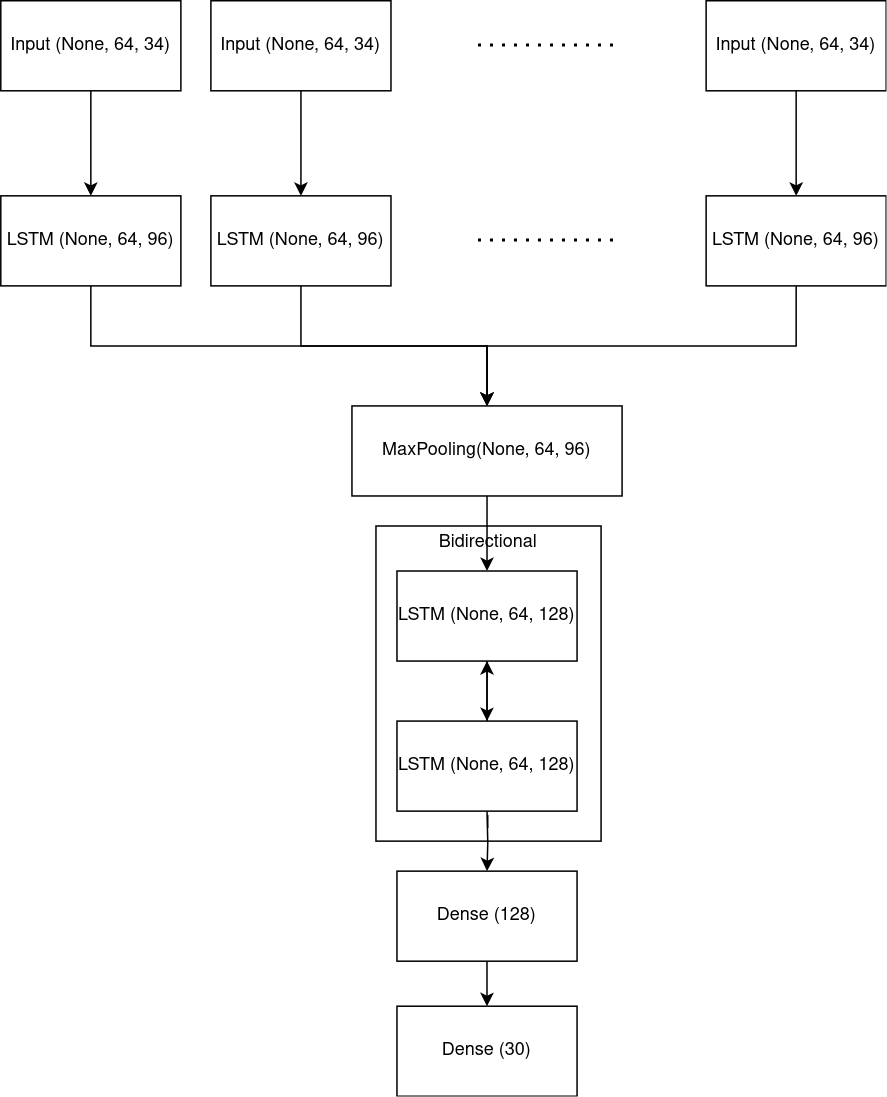
\includegraphics[width=0.70\linewidth]{skeletons-arch.png}
    \caption{Architektura hierarchicznego modelu czasowego opartego o szkielety uczestników akcji, z warstwą dwukierunkową LSTM}
    \label{fig:skeletons-arch}
\end{figure}

\subsubsection{Wyniki} 
Skuteczność hierarchicznego modelu opartego na cechach szkieletowych wyniosła 41.52\% , wyliczona w tabeli \ref{tab:szkielety-wyniki}. Na tak niską skuteczność składa się kilka czynników: \begin{itemize}
    \item Same szkielety niosą informację tylko i wyłącznie o ruchach poszczególnych osób, tracony jest cały pozostały kontekst akcji tj. tło, ubiór, sprzęt.
    \item Czynności wykonywane w sporcie mają bardzo duży wspólny podzbiór ruchów np. aktywność biegania występuje w prawie wszystkich sportach lekkoatletycznych. 
    \item W danych szkieletowych wyekstrahowanych przez model występuje szum związany z trudnością przetworzenia nagrań, do których dochodzą niestandardowe dla modelu pozy występujące w sporcie. 
\end{itemize}
\begin{table}[!h]  \centering
\caption{Wyniki modelu opartego na cechach szkieletowych}
\begin{tabular} {| c | c | c | c | r |} \hline
    Model & Podział 1.  & Podział 2. & Podział 3. & \textbf{Średnia} \\ \hline\hline
    Hierarchiczny model szkieletowy &  39.81\%	& 42.72\%	& 42.03\% & \textbf{41.52\%} \\ \hline
\end{tabular}
    \label{tab:szkielety-wyniki}
\end{table}
Ze względu na niską skuteczność modelu, badania modeli opartych wyłącznie na cechach szkieletowych zostały porzucone. 

\subsection{Hierarchiczne modele RGB}
\subsubsection{Hierarchiczny model RGB z warstwą MaxPoolingu}
Hierarchiczny model oparty na cechach RGB, oparty jest na tych samych założeniach oraz tej samej architekturze co model szkieletowy, różni się jedynie wejściem modelu, zamiast szkieletów działa na cechach RGB wyekstrahowanych przy pomocy modelu MobileNetV3 \cite{mobilenet}. Wraz ze zmianą wejścia konieczne jest również dostosowanie rozmiarów warstw. Architektura jest reimplementacją architektury przedstawionej w pracy Ibrahim et al. \cite{Ibrahim2015}, zmienione uległy wielkości warstw, ponieważ wektory wejściowe zostały uzyskane w inny sposób. Dla danej architektury, tak samo jak dla cech szkieletowych lepsze wyniki dało zastąpienie pojedynczej warstwy LSTM  dwoma warstwami połączonymi dwukierunkowo dla kodowania sekwencji. Architektura modelu została przedstawiona na rysunku \ref{fig:sp-arch}. Całkowita ilość trenowalnych parametrów modelu wynosi 450 974. 
\begin{figure}[!h]
    \centering 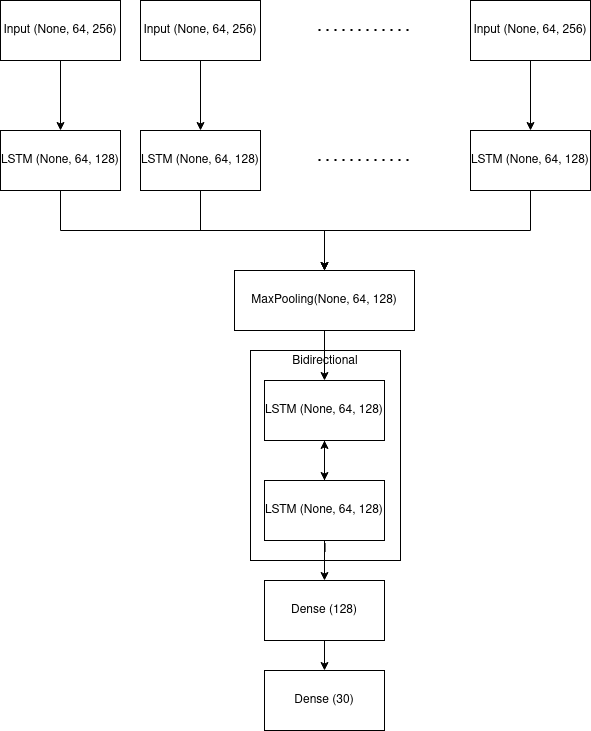
\includegraphics[width=0.70\linewidth]{sp-arch.png}
    \caption{Architektura hierarchicznego modelu czasowego opartego o cechy RGB uczestników akcji, z warstwą dwukierunkową LSTM}
    \label{fig:sp-arch}
\end{figure}

\subsubsection{Hierarchiczny model RGB z warstwą konkatenacji}
Przetestowana została również autorska modyfikacja modelu hierarchicznego. Eksperyment polegał na zastosowaniu dwóch dwukierunkowych warstw LSTM do zakodowania sekwencji pojedynczych osób oraz zastąpieniem warstwy MaxPooling'u warstwą konkatenacji. Pierwsza zmiana wynikała z obserwacji dokonanej w trakcie treningu, mówiącej, że dwukierunkowy LSTM daje lepsze wyniki dla zadania kodowania sekwencji aktywności. Druga zmiana wynikała z wątpliwości, że dokonując max-poolingu utracona zostaje zbyt duża ilość informacji, poprzez konkatenacje badana jest skuteczność modelu dysponująca wszystkimi przekazanymi do niego danymi. Architektura modelu przedstawiona została na rysunku \ref{fig:sp-con-arch}. Liczba trenowalnych parametrów modelu wynosi 547 774. 
\begin{figure}[!h]
    \centering 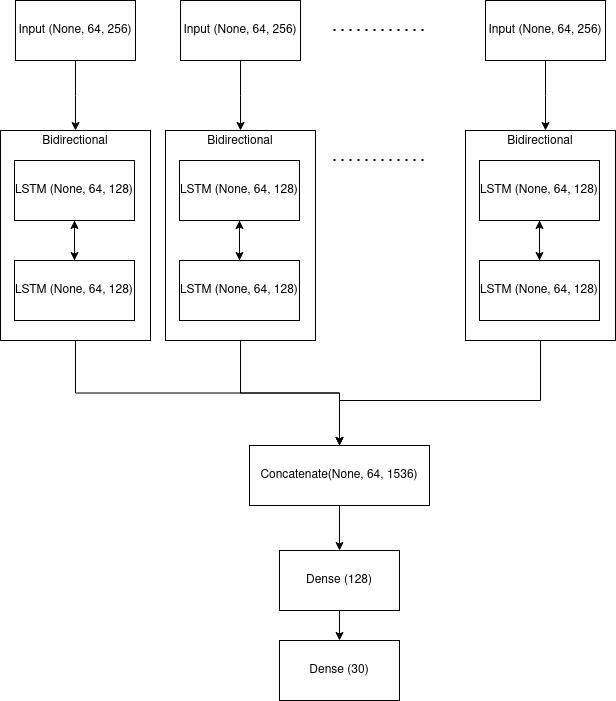
\includegraphics[width=0.70\linewidth]{sp-con-arch.png}
    \caption{Architektura hierarchicznego modelu czasowego opartego o cechy RGB uczestników akcji, ze zrównolegloną warstwą dwukierunkową LSTM oraz warstwą konkatenacji}
    \label{fig:sp-con-arch}
\end{figure}

\subsubsection{Wyniki}
Hierarchiczne modele oparte na cechach RGB osiągnęły skuteczności 62.48\%, 69.38\% wyliczone w tabeli \ref{tab:hier-rgb-wyniki}. Zastąpienie cech szkieletowych cechami RGB dało wysoką poprawę rzędu 20 punktów procentowych. Model ten rozwiązuje część problemów, które występują dla danych szkieletowych, posiada informację o ruchach poszczególnych osób, oraz części obrazu, jednak nie posiada informacji o tle oraz miejscu wykonywanej akcji. 

Wyniki uzyskane przez model wykorzystujący warstwę Max-Pooling'u są zbliżone do wyników, które uzyskał Ibrahim et al. \cite{Ibrahim2015} dla trudniejszego zbioru, które wynoszą 51.1\%. Zastąpienie warstwy Max-Pooling'u warstwą konkatenacji, oraz zepchnięcie dwukierukierunkowej warstwy LSTM do analizy akcji pojedynczych osób poprawiło skuteczność modelu o około 8 punktów procentowych, potwierdzając hipotezę o bardzo dużej utracie danych związanych z redukcją wymiaru. 
\begin{table}[!h] \centering
\caption{Wyniki modelów hierarchicznych opartych na cechach RGB}
\begin{tabular} {| c | c | c | c | r |} \hline
    Model & Podział 1.  & Podział 2. & Podział 3. & \textbf{Średnia} \\ \hline\hline
    Hierarchiczny model RGB &  61.42\%	& 62.47\%	& 63.56\%	& \textbf{62.48\%} \\ \hline
    Hierarchiczny model RGB z konkatenacją &  68.82\%	& 68.58\%	& 70.74\%	& \textbf{69.38\%} \\ \hline
\end{tabular}
\label{tab:hier-rgb-wyniki} 
\end{table}

\subsection{Model badający cały obraz}
Przeprowadzone również zostały eksperymenty modelu działającym na całych klatkach nagrania, bez wyznaczania poszczególnych osób. Wejściem do modelu jest sekwencja długości $T$, uzyskana w sposób opisany w rozdziale \ref{sekwncje-klatek}. Wejście przekazywane jest dwukierunkowej sieci LSTM, takiej samej jak we wszystkich wcześniej przedstawionych modelach, następnie do dwóch warstw gęstych oraz warstwy klasyfikacyjnej. Architektura przedstawiona została na rysunku \ref{fig:frame-arch}. Całkowita liczba trenowalnych parametrów modelu wynosi 435 710. 
\begin{figure}[!h]
    \centering 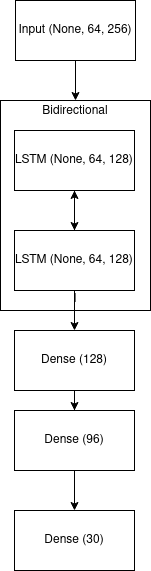
\includegraphics[width=0.2\linewidth]{frame-arch.png}
    \caption{Architektura modelu czasowego opartego o cechy RGB klatek nagrania}
    \label{fig:frame-arch}
\end{figure}
\subsubsection{Wyniki}
Model badający cały obraz osiągnął skuteczność 76.16\%, wyliczone w tabeli \ref{tab:frame-rgb-wyniki}. Wynik ten udowadnia, że  globalne cechy obrazu niosą więcej informacji niż same akcje poszczególnych osób na nagraniu. 
\begin{table}[!h] \centering
\caption{Wyniki}
\begin{tabular} {| c | c | c | c | r |} \hline
    Model & Podział 1.  & Podział 2. & Podział 3. & \textbf{Średnia} \\ \hline\hline
    Model klatkowy &  78.10\%	& 74.88\%	& 75.49\%	& \textbf{76.16\%} \\ \hline
\end{tabular}
\label{tab:frame-rgb-wyniki} 
\end{table}
\subsection{Fuzja modeli} 
Dysponując dużą liczbą modeli, działających na różnych cechach przetestowane zostało również wielomodelowe rozwiązanie problemu poprzez dokonanie późnej fuzji modeli, które osiągnęły najlepszą skuteczność dla konkretnego rodzaju danych, z modelem działającym na całym obrazie. Eksperyment ten ma na celu rozszerzenie kontekstu na jakim działa model badający cały obraz o więcej informacji o akcjach poszczególnych osób. Badane modele razem z wynikami przedstawione zostały w tabeli \ref{tab:fuzja-wyniki}. 

Późna fuzja wykonana została poprzez odrzucenie z łączonych ze sobą modeli ostatniej warstwy gęstej (głowy modelu), oraz konkatenację wyjściowych logitów z wyjściowej warstwy gęstej i przekazanie ich do nowej głowy modelu (warstwy gęstej o liczbie neuronów równej liczbie klas). Na rysunku \ref{fig:fuse-example-arch} przedstawiona została fuzja modelu działającego na całych klatkach \ref{fig:frame-arch} z modelem hierarchicznym \ref{fig:sp-con-arch}. Połączone ze sobą modele trenowane są w całości od nowa. 


\begin{figure}[!h]
    \centering 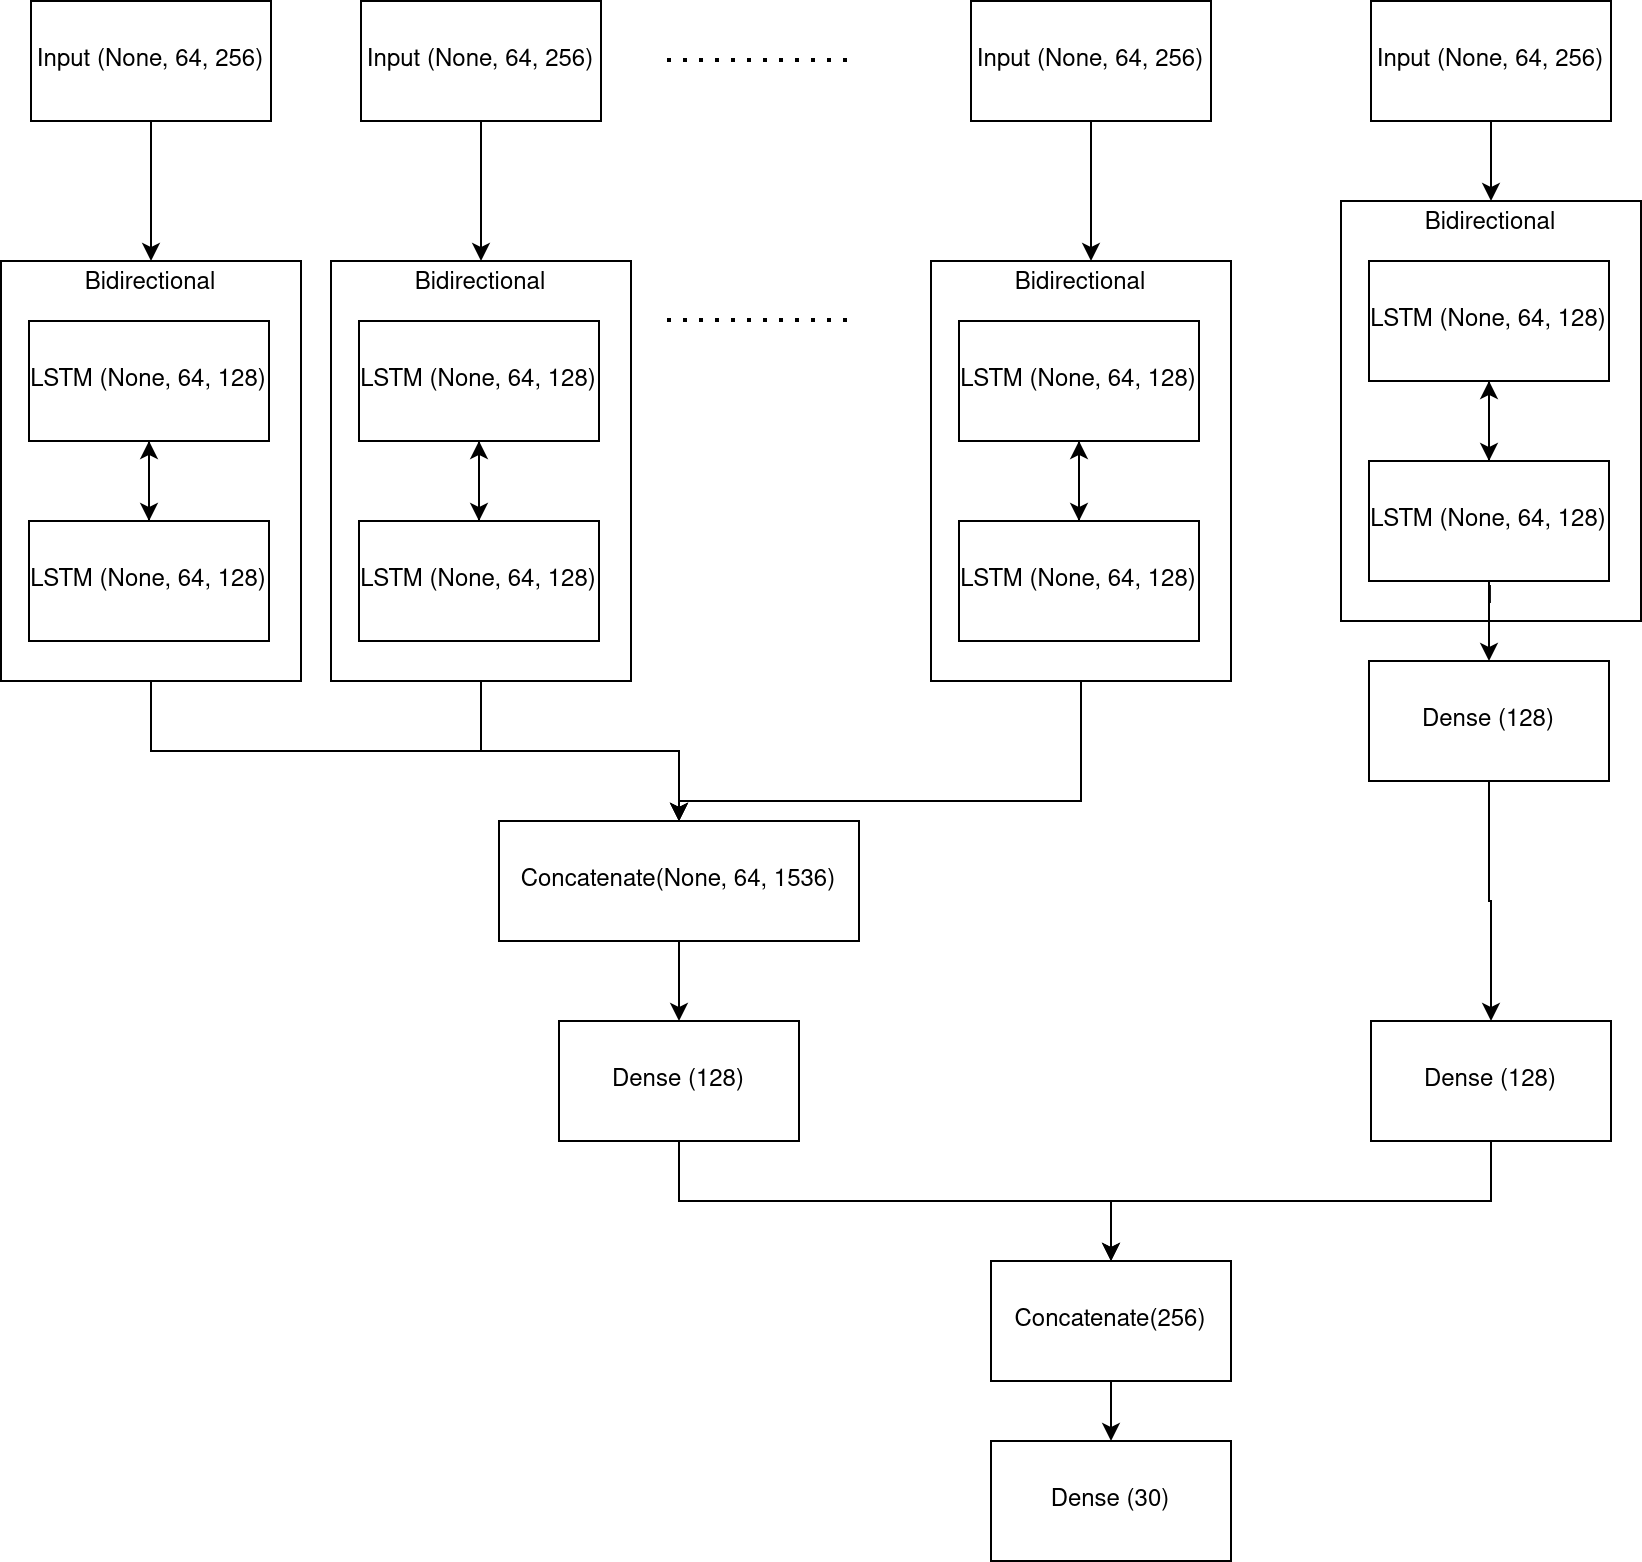
\includegraphics[width=0.70\linewidth]{fuse-example.png}
    \caption{Architektura hierarchicznego modelu czasowego opartego o cechy RGB uczestników akcji, ze zrównolegloną warstwą dwukierunkową LSTM oraz warstwą konkatenacji}
    \label{fig:fuse-example-arch}
\end{figure}

\subsubsection{Wyniki} \label{najlepszy-model}
Wyniki fuzji z konkretnymi modelami zostały przedstawione w tabeli \ref{tab:fuzja-wyniki}. 

Fuzja modelu szkieletowego z modelem klatkowym daje pomijalną poprawę wynoszącą około 1 punktu procentowego. Niski poziom poprawy spowodowany jest prawdopodobnie niską skutecznością samego modelu szkieletowego, która została wykazana we wcześniejszym eksperymencie. Najprawdopodobniej model w dużej mierze ignoruje wkład szkieletowy oraz predykcji dokonuje wzorując się tylko na klatkach nagrania. 

Fuzja modelu hierarchicznego opartego na cechach RGB z modelem klatkowym przyniosła wysoką poprawę wynoszoną około 5 punktów procentowych. W tym przypadku model zgodnie z wcześniej postawioną hipotezą, korzysta z rozszerzonego kontekstu. Jest to również model o najlepszej skuteczności opisany w tej pracy. Zostanie wykorzystany do porównań z modelami referencyjnymi na tym zbiorze. 

Fuzja wszystkich trzech modelów daje statystycznie nieistotny rezultat w porównaniu do fuzji hierarchicznego modelu RGB oraz modelu klatkowego. Fuzja z modelem szkieletowym nie daje istotnej poprawy skuteczności. 
\begin{table}[!h] \centering
\caption{Wyniki modeli po fuzji.}
\begin{tabular} {| c | c | c | c | r |} \hline
    Model & Podział 1.  & Podział 2. & Podział 3. & \textbf{Średnia} \\ \hline\hline
    \begin{tabular}[c]{@{}l@{}}Hierarchiczny model szkieletowy +\ \ \ \ \ \ \ \ \ \ \ \ \ \ \ \ \ \\ Model klatkowy\end{tabular} &  77.82\%	& 76.18\%	& 78.19\%	& \textbf{77.40\%} \\ \hline
    \begin{tabular}[c]{@{}l@{}}Hierarchiczny model RGB z konkatenacja +\\ Model klatkowy\end{tabular} &  82.65\%	& 79.24\%	& 79.68\%	& \textbf{80.53\%} \\ \hline
    \begin{tabular}[c]{@{}l@{}}Hierarchiczny model szkieletowy +\\ Hierarchiczny model RGB z konkatenacja +\\ Model klatkowy\end{tabular}&  80.76\%	& 78.78\%	& 81.27\%	& \textbf{80.27\%} \\ \hline
\end{tabular}
\label{tab:fuzja-wyniki} 
\end{table}
\subsection{Interpretacja wyników modelu} 
W tej sekcji opisana została interpretacja wyników zwracanych przez najlepszy znaleziony model w eksperymentach 
\ref{najlepszy-model}. Macierz pomyłek modelu przedstawiona została na rysunku \ref{fig:conf-matrix}. Model skutecznie 
nauczył się rozpoznawać większość klas. Najbardziej problematyczne sporty zostały opisane poniżej.
\begin{figure}[!h]
    \centering 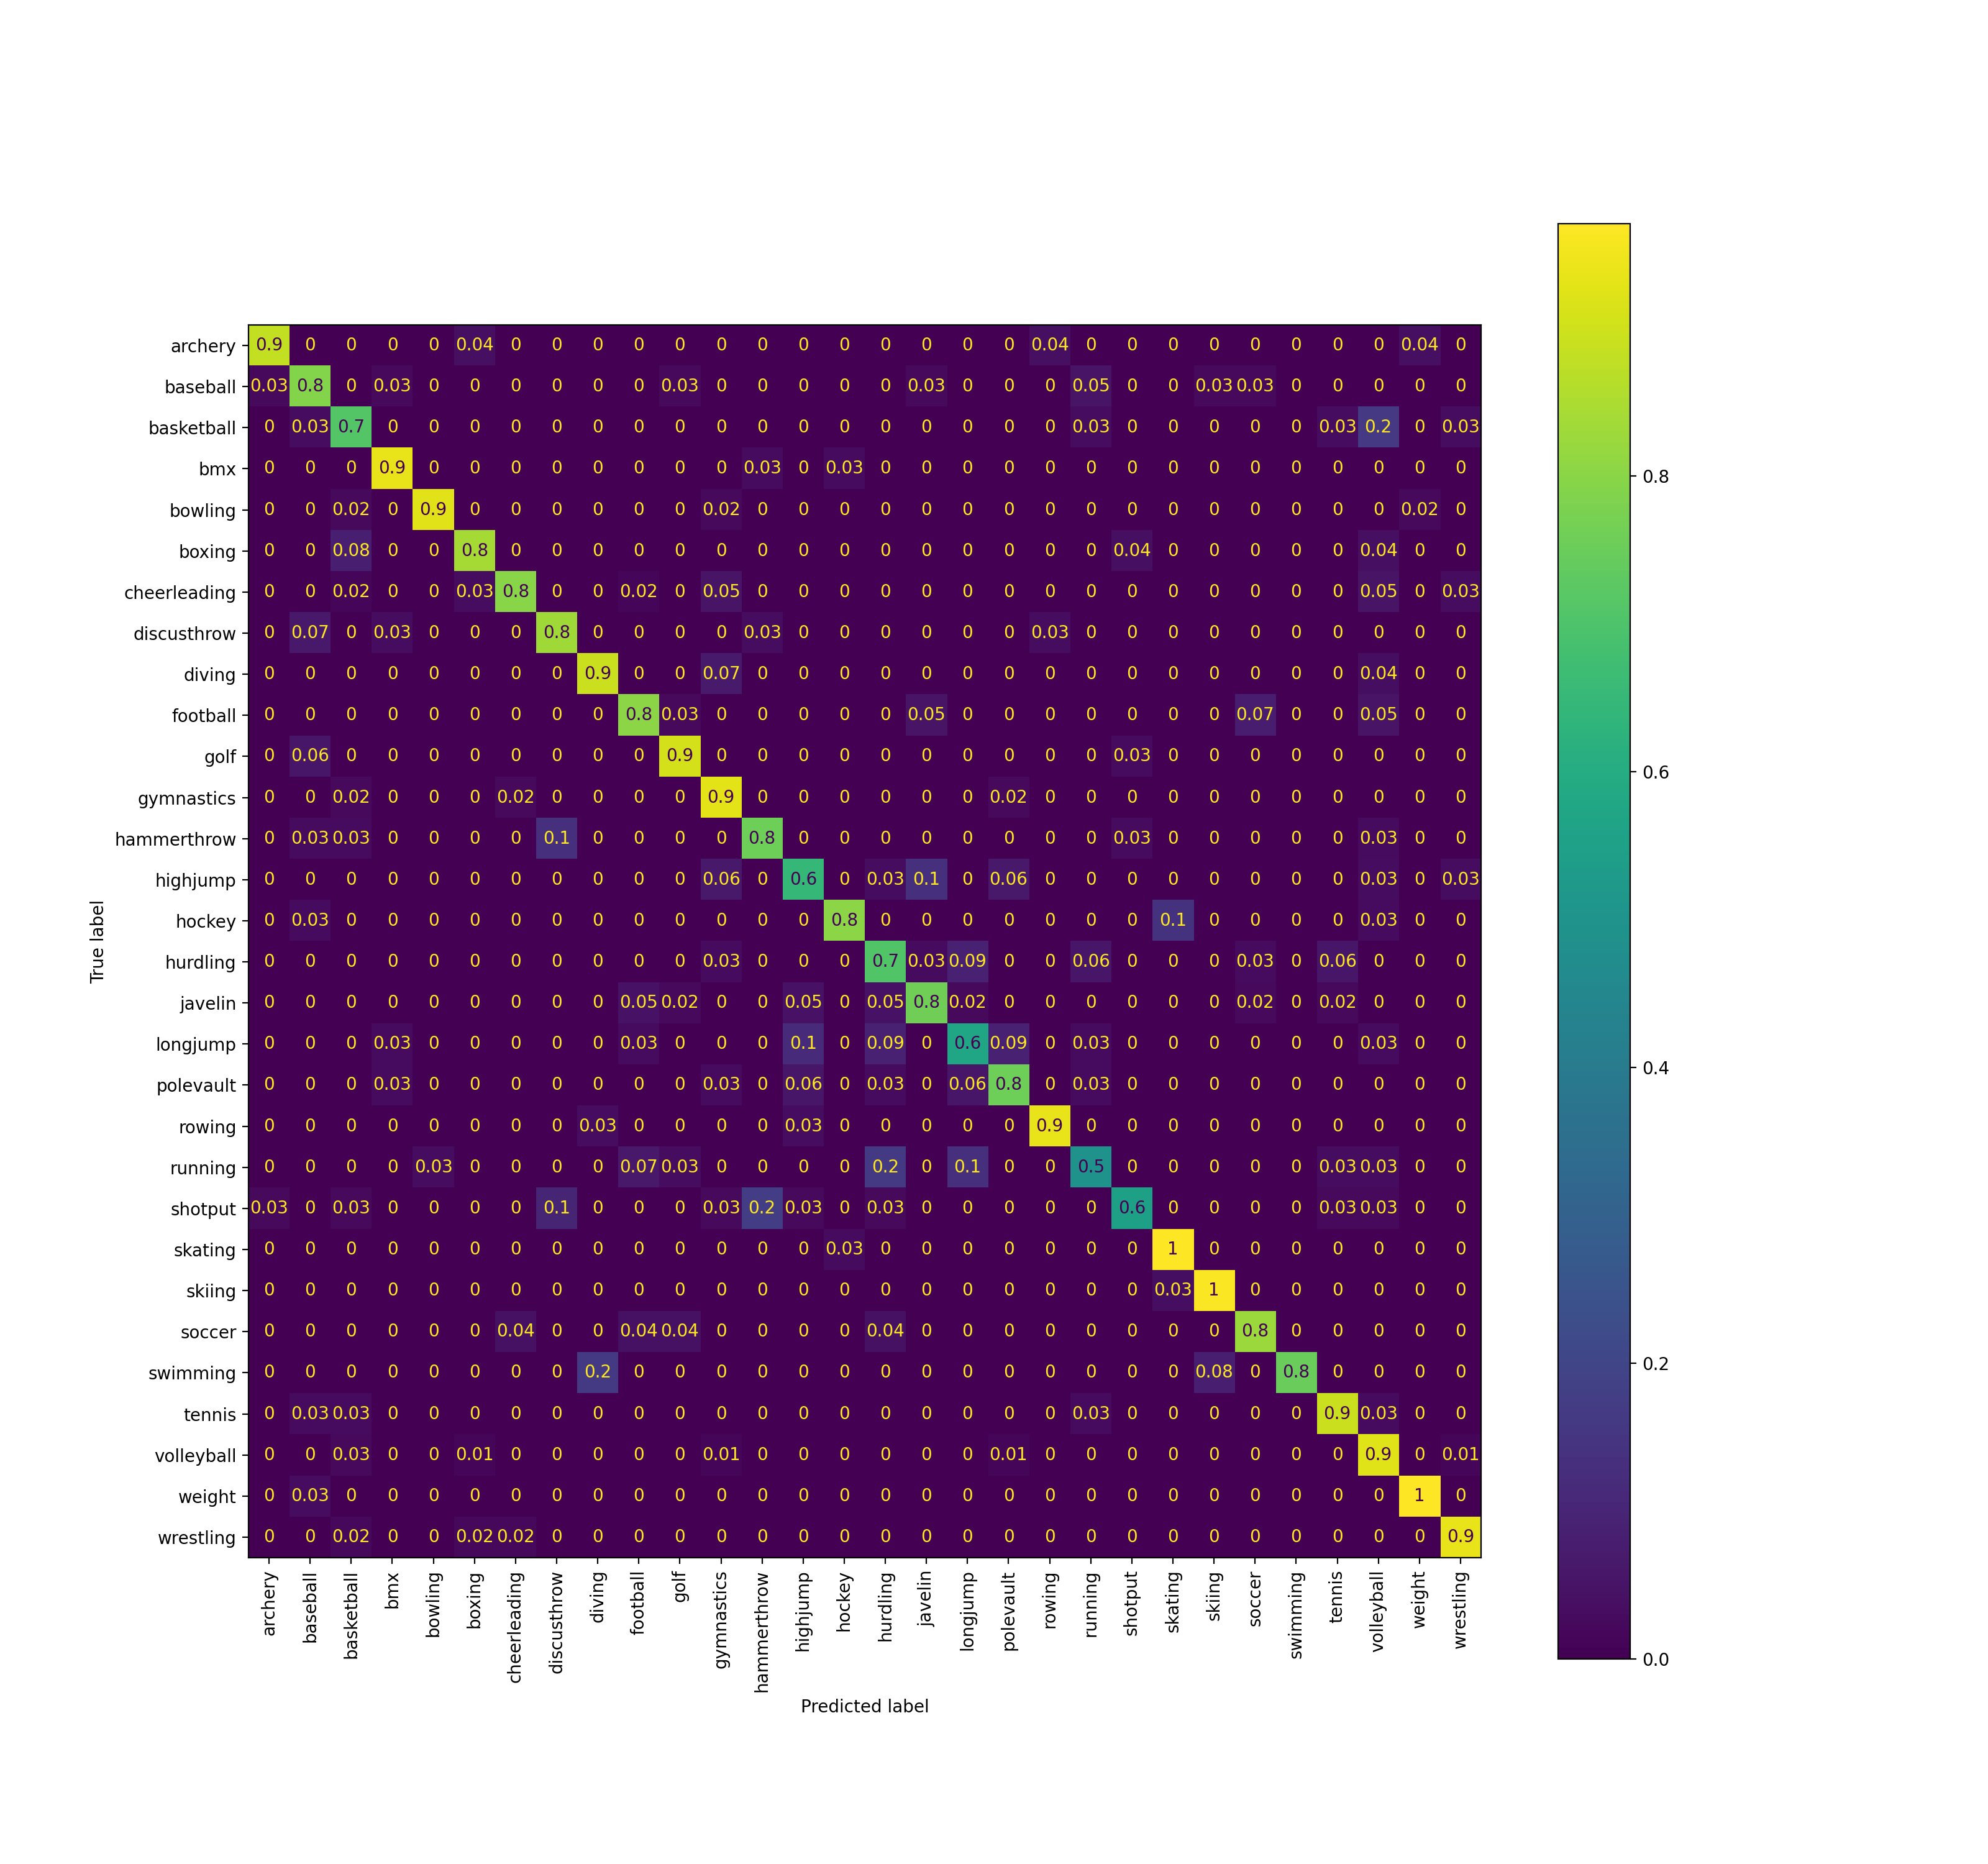
\includegraphics[width=0.99\linewidth]{confusion_matrix.png}
    \caption{Macierz pomyłek najlepszego znalezionego modelu}
    \label{fig:conf-matrix}
\end{figure}
\subsubsection{Wariacje biegania} 
Model ma największy problem z rozpoznawaniem sportów będącymi wariacjami biegania np. bieg przez płotki oraz sportami,
których dużą częścią jest wykonanie rozbiegu np. skok w dal. W pierwszym przypadku model ma problem z rozpoznawaniem 
innej techniki biegu. Drugim problemem jest zastosowanie próbkowania nagrań wideo opisanego w sekcji 
\ref{klasyfikacja}. Dla sportów tj. skok w dal, w których dużą część stanowi wzięcie rozbiegu większość próbek, 
będzie klasyfikowana jako bieg, a część kluczowa, czyli sam skok stanowi mniejszość próbek, przez co nie będą one w 
stanie stanowić przeciwwagi dla wcześniejszych predykcji. 
\subsubsection{Rzuty}
Kolejnym widocznym problemem modelu są rzuty tj. rzut kulą, rzut młotem, rzut dyskiem. Problem rozpoznania tych klas 
wynika z bardzo zbliżonej techniki wykonywanego sportu oraz otoczenia, w jakim wykonuje się sport, czyli klatki z siatki. 
\subsubsection{Koszykówka - Siatkówka}
Pomyłki modelu dla tych dwóch kategorii najprawdopodobniej wynikają z rodzajów boiska, 
na którym wykonywany jest sport oraz podobnych ruchów wykonywanych przez zawodników. W dużej mierze nagrania wchodzące 
w skład zbioru danych przedstawiają treningi wykonywane na sali gimnastycznej przygotowanej do ogólnego użytku (w tle 
znajdują się rozwieszone kosze do gry w koszykówkę). Część ruchów wykonywanych przez zawodników w tych sportach jest 
również bardzo podobna, a nawet taka sama np. blok. 